\documentclass[11pt]{article}

\usepackage[margin=0.85in]{geometry}
\usepackage{booktabs}
\usepackage{tabularx}
\usepackage{array}
\usepackage{amsmath}
\usepackage{graphicx}
\usepackage{xcolor}
\usepackage{enumitem}
\usepackage{microtype}
\usepackage{fancyhdr}
\usepackage{hyperref}
\usepackage{caption}
\usepackage{setspace}

\hypersetup{
  colorlinks=true,
  linkcolor=blue!55!black,
  urlcolor=blue!60!black,
  citecolor=blue!55!black
}

\pagestyle{fancy}
\fancyhf{}
\lhead{\small Exposure \& Aging Context Note}
\rhead{\small Laidlaw / HKU}
\cfoot{\thepage}
\renewcommand{\headrulewidth}{0.3pt}

\setlength{\parindent}{0pt}
\setlength{\parskip}{0.55em}
\setlist[itemize]{leftmargin=1.35em, itemsep=0.2em, topsep=0.25em}
\setlist[enumerate]{leftmargin=1.5em, itemsep=0.2em, topsep=0.25em}
\captionsetup{font=small, labelfont=bf, skip=6pt}

\newcommand{\realdata}{\textcolor{green!35!black}{\textbf{Real data}}}
\newcommand{\pending}{\textcolor{red!60!black}{\textbf{Pending}}}

\title{
  \textbf{Exposure and Demographic Context}\\[0.35em]
  \large Official Thermal Extremes and Population Aging in Hong Kong, 2013--2023\\[0.4em]
  \normalsize\textit{A Laidlaw Scholars deliverable preceding Hospital Authority outcome analysis}
}
\author{
  Bob Shen Ruililin\\
  Laidlaw Scholars Programme, The University of Hong Kong\\[0.35em]
  \small
  Supervisor: Professor David Bishai\\
  Collaborators: Hogan (environment); Roro (Hospital Authority access)
}
\date{11 July 2026}

\begin{document}
\maketitle

\begin{center}
\small\textit{
This note reports only what can be defended with public data already in hand.
It does not estimate associations between temperature and cardiovascular admissions.
Those analyses await an approved Hospital Authority extract.
}
\end{center}

\section*{Positioning statement}

As Laidlaw Scholars we are accountable for two things at once: intellectual ambition and
evidentiary honesty. The wider project asks how officially defined thermal extremes---especially
hot nights and cold days---relate to cardiovascular hospital burden in an aging Hong Kong.
That question cannot be answered without clinical outcomes. What \emph{can} be answered now,
rigorously, is whether the environmental and demographic setting of 2013--2023 contains the
contrast the study design requires, and whether that setting supports a coexistence framing
rather than a ``heat replaced cold'' narrative.

This deliverable therefore ships three products: (i)~validated official extreme-day series at
the Hong Kong Observatory (HKO) Headquarters; (ii)~a spell-structure decomposition of those
extremes; and (iii)~Census and Statistics Department (C\&SD) mid-year population change in
intervention-relevant older age bands. All three are \realdata{}. Hospital Authority (HA)
outcomes remain \pending{}.

\section{Scientific framing}

Earlier Hong Kong daily studies found cold-dominant cardiovascular associations
\citep{goggins2013,goggins2012}. Recent work shows that official binary hot nights may be a
weak biological metric relative to nighttime heat intensity \citep{guo2024}, while consecutive
extreme events carry additional mortality information \citep{wang2019}. Our planned monthly
design estimates hospital \emph{burden}, not daily triggering; coefficients will not be
numerically comparable to Goggins-era per-$^\circ$C rate ratios.

Against that literature, the present note asks a narrower, prior question:

\begin{quote}
\textit{Do contemporary Hong Kong thermal extremes and age structure provide meaningful
exposure and demographic contrast for a 2013--2023 monthly study that keeps both heat and
cold in view?}
\end{quote}

A negative answer would argue for redesign. A positive answer does not prove a heat effect;
it justifies proceeding to outcome analysis without overclaiming.

\section{Data and methods}

\subsection{Thermal extremes}

Daily HKO Headquarters observations were parsed from official \texttt{dailyExtract} files and
aggregated to calendar months. Official definitions were applied without modification:

\begin{center}
\begin{tabular}{@{}ll@{}}
\toprule
Metric & Definition \\
\midrule
Hot night & Daily minimum temperature $\ge 28^\circ$C \\
Very hot day & Daily maximum temperature $\ge 33^\circ$C \\
Extremely hot day & Daily maximum temperature $\ge 35^\circ$C \\
Cold day & Daily minimum temperature $\le 12^\circ$C \\
\bottomrule
\end{tabular}
\end{center}

Months with temperature completeness below 90\% would have extreme counts set to missing;
no such months occurred in the core window. Annual totals for hot nights, very hot days, and
cold days were compared with HKO \textit{The Year's Weather} summaries for 2013--2023:
\textbf{33 of 33 annual checks matched}.

Spell metrics follow the spirit of Wang et al.\ \citep{wang2019}: days belonging to runs of
five or more consecutive hot nights (or very hot days), and months touched by a simple
2D3N-type window (at least two very hot days and three hot nights within five days). These
are descriptive exposure engineering, not causal claims.

\subsection{Population}

Mid-year population by sex and five-year age group was imported from C\&SD Table 110-01001
(MDT public file; values in thousands converted to persons). Ages 65--69 and 70--74 are kept
separate, following collaborator advice that these cohorts are both growing and practically
reachable for intervention. Aging contrasts use exact mid-year counts for 2013 and 2023.

\subsection{What this note deliberately excludes}

\begin{itemize}
  \item Any Hospital Authority admission counts or model coefficients.
  \item Placeholder air-pollution series (awaiting real EPD imports and Hogan quality review).
  \item Claims that heat has replaced cold, or that climate change has already shifted the
        cardiovascular risk regime.
\end{itemize}

\section{Results}

\subsection{Thermal extremes: rising heat, persistent cold}

Figure~\ref{fig:annual} shows annual counts of hot nights, very hot days, and cold days.
Hot nights rose from 10 in 2013 to 61 in 2021 (56 in 2023). Very hot days rose from 17 to
54 over the same 2013--2021 comparison. Cold days did not disappear: 14 in 2013, 13 in 2021,
and 14 in 2023.

\begin{figure}[htbp]
  \centering
  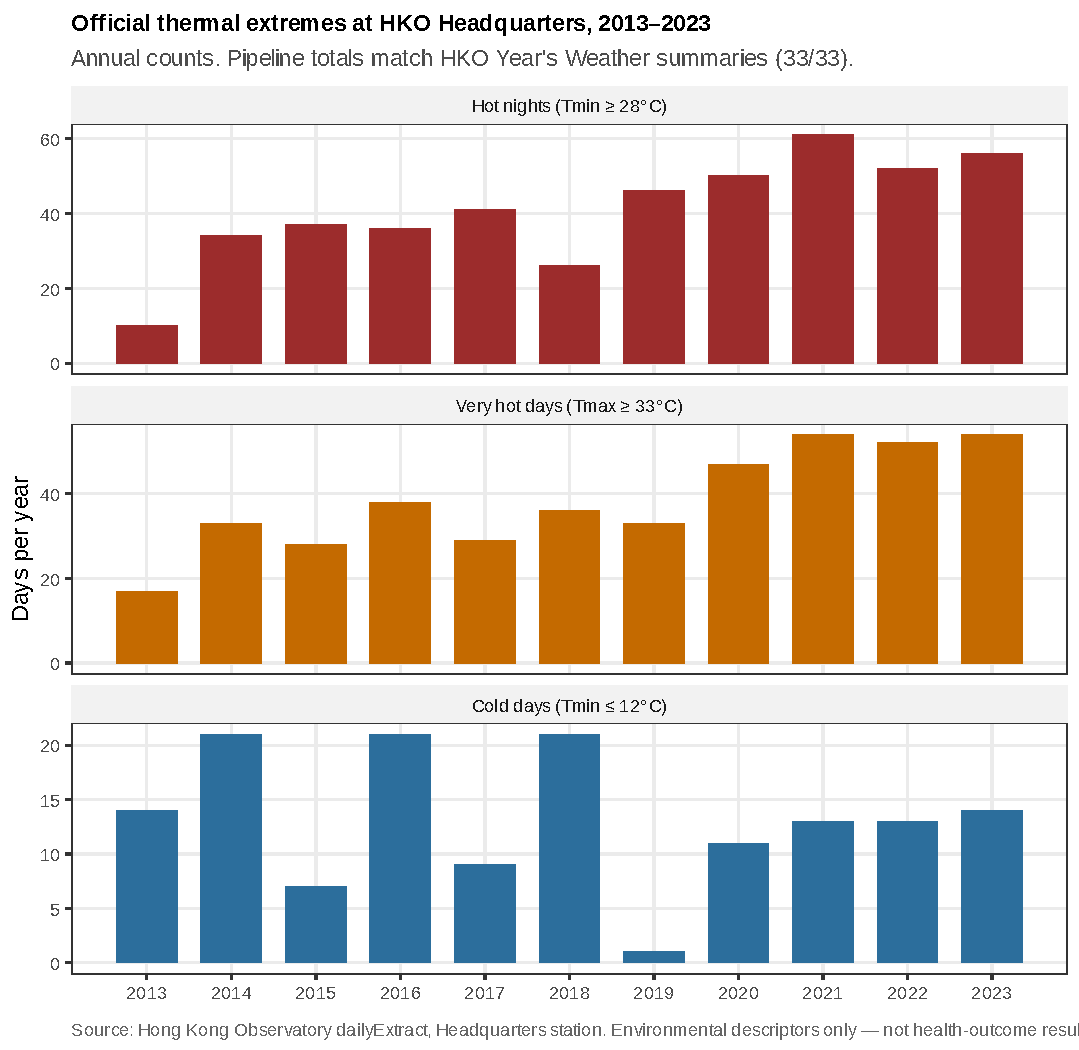
\includegraphics[width=0.92\textwidth]{../../figures/exposure_aging/fig01_annual_extremes_coexistence.pdf}
  \caption{Annual official thermal extremes at HKO Headquarters, 2013--2023.
  Pipeline annual totals match HKO \textit{Year's Weather} summaries for all 33 checks.
  These are environmental exposure descriptors, not health-outcome results.}
  \label{fig:annual}
\end{figure}

Period means sharpen the contrast without implying a formal trend test
(Table~\ref{tab:period}). Mean annual hot nights increased from 30.7 (2013--2018) to 53.0
(2019--2023). Mean cold days declined from 15.5 to 10.4 but remained non-trivial. The
scientific implication is coexistence with changing weights---not succession.

\begin{table}[ht]
\centering
\caption{Period means of annual extreme counts, HKO Headquarters}
\label{tab:period}
\small
\begin{tabular}{@{}lcccc@{}}
\toprule
Period & Years & Mean hot nights & Mean very hot days & Mean cold days \\
\midrule
2013--2018 & 6 & 30.7 & 30.2 & 15.5 \\
2019--2023 & 5 & 53.0 & 48.0 & 10.4 \\
\bottomrule
\end{tabular}
\end{table}

Figure~\ref{fig:monthly} shows the same coexistence at monthly resolution. Hot-night bars
intensify in the later period; cold-day lines continue to appear in winter months of warm
years. For a monthly burden model, this pattern supplies exposure variation on both margins.

\begin{figure}[htbp]
  \centering
  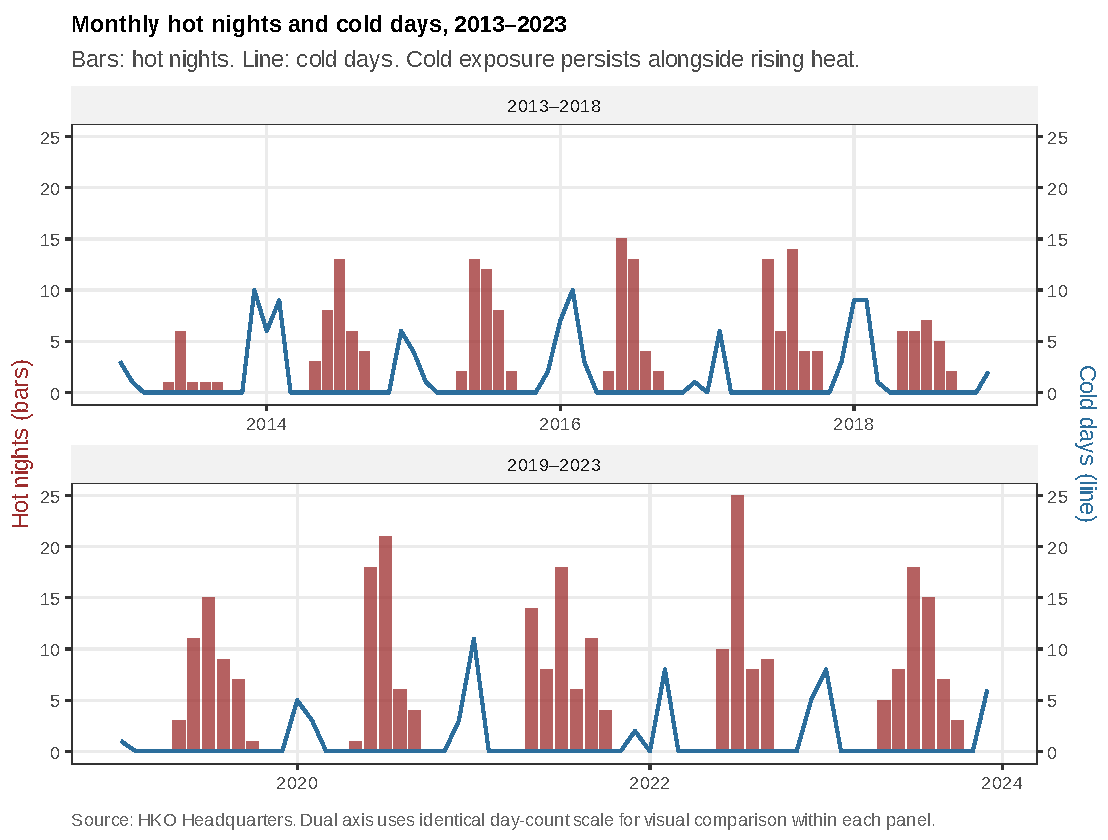
\includegraphics[width=0.94\textwidth]{../../figures/exposure_aging/fig02_monthly_hot_nights_cold_days.pdf}
  \caption{Monthly hot nights (bars) and cold days (line), 2013--2023, split by period.
  Cold days remain visible alongside the later rise in hot nights.}
  \label{fig:monthly}
\end{figure}

\subsection{Spell structure: extremes are not only scattered counts}

Monthly totals discard sequence. Across 2013--2023, on average about 42\% of annual hot
nights fell inside spells of five or more consecutive nights (Figure~\ref{fig:spell}).
That share was higher in 2019--2023 (mean 0.51) than in 2013--2018 (mean 0.34). Months
touched by a 2D3N-type window also rose (means 2.7 vs 4.4 months per year).

\begin{figure}[htbp]
  \centering
  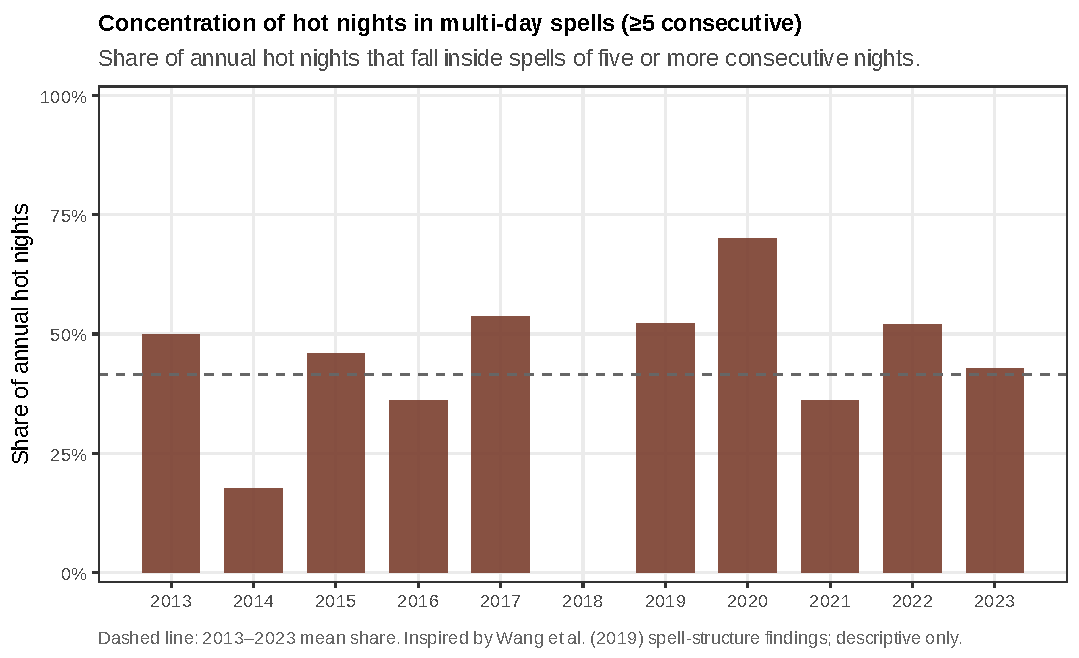
\includegraphics[width=0.92\textwidth]{../../figures/exposure_aging/fig03_hot_night_spell_concentration.pdf}
  \caption{Share of annual hot nights occurring inside consecutive spells of length
  $\ge 5$. Dashed line: 2013--2023 mean. Descriptive exposure structure only.}
  \label{fig:spell}
\end{figure}

We read this cautiously. Spell concentration motivates retaining spell and combination
metrics as \emph{prespecified alternatives} to official binary counts---especially given
Guo et al.'s finding that binary HNday28 may not track hospitalization risk while intensity
does \citep{guo2024}. A null monthly association for official hot-night counts would be
compatible with that literature and would not close the nighttime-heat question.

\subsection{Population aging: 65--69 and 70--74 nearly doubled}

C\&SD mid-year counts show rapid growth in the older bands prioritized by the team
(Table~\ref{tab:aging}; Figures~\ref{fig:aging}--\ref{fig:older}). Ages 65--69 rose from
295{,}100 in mid-2013 to 568{,}500 in mid-2023 (+92.6\%). Ages 70--74 rose from 213{,}100
to 424{,}800 (+99.3\%). Ages 85+ grew by 63.9\%. Several mid-life bands were flat or
declining.

\begin{table}[ht]
\centering
\caption{Mid-year population in older age groups, C\&SD Table 110-01001 (both sexes)}
\label{tab:aging}
\small
\begin{tabular}{@{}lrrrr@{}}
\toprule
Age group & Mid-2013 & Mid-2023 & Absolute change & \% change \\
\midrule
65--69 & 295{,}100 & 568{,}500 & +273{,}400 & +92.6 \\
70--74 & 213{,}100 & 424{,}800 & +211{,}700 & +99.3 \\
75--79 & 210{,}200 & 254{,}100 & +43{,}900 & +20.9 \\
80--84 & 157{,}600 & 158{,}600 & +1{,}000 & +0.6 \\
85+ & 143{,}900 & 235{,}900 & +92{,}000 & +63.9 \\
\bottomrule
\end{tabular}
\end{table}

\begin{figure}[htbp]
  \centering
  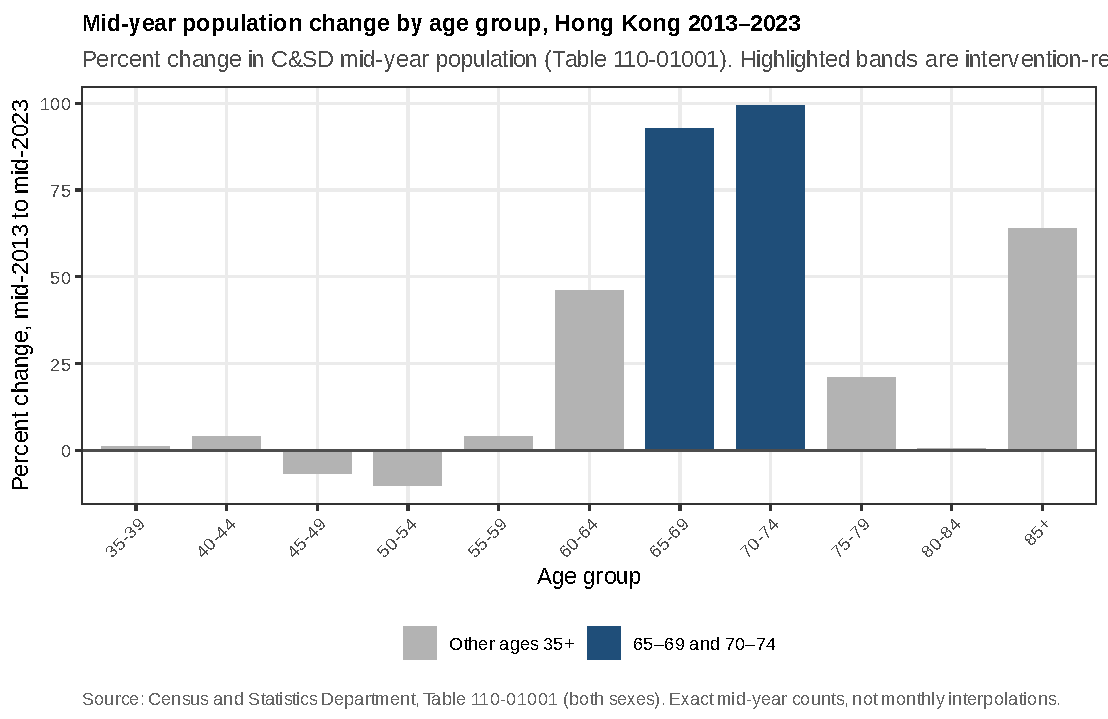
\includegraphics[width=0.94\textwidth]{../../figures/exposure_aging/fig04_population_aging_pct_change.pdf}
  \caption{Percent change in mid-year population by age group, 2013--2023.
  Ages 65--69 and 70--74 are highlighted as intervention-relevant cohorts.}
  \label{fig:aging}
\end{figure}

\begin{figure}[htbp]
  \centering
  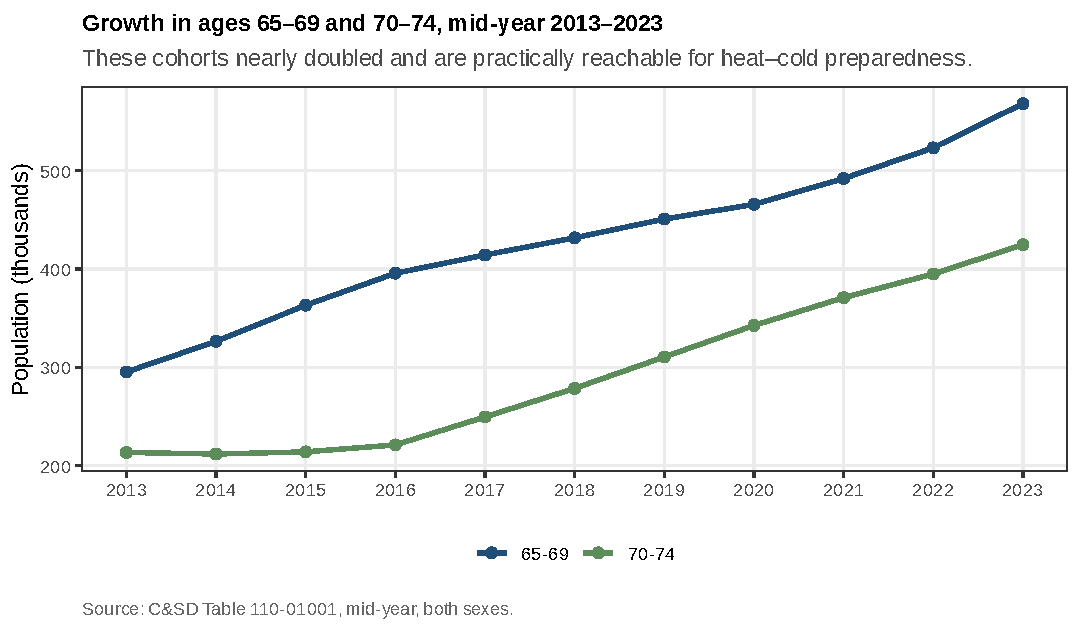
\includegraphics[width=0.92\textwidth]{../../figures/exposure_aging/fig05_older_cohorts_timeseries.pdf}
  \caption{Mid-year population trajectories for ages 65--69 and 70--74, 2013--2023.}
  \label{fig:older}
\end{figure}

For the eventual admission analysis, these denominators are not decorative. Raw counts of
AMI or stroke admissions cannot be interpreted as changing risk while the older population
nearly doubles. The planned offset---$\log(\text{age--sex population}\times\text{days in
month})$---is therefore a scientific requirement, not a modelling flourish.

\section{Reflective synthesis}

Three conclusions follow from public data alone.

\paragraph{1. The exposure window is analytically usable.}
2013--2023 is not a uniformly hot decade. It contains substantial heat contrast and
retained cold days. A monthly model has something to estimate on both margins.

\paragraph{2. Coexistence is the honest framing.}
Cold days in high-heat years (for example 13 cold days alongside 61 hot nights in 2021)
make a ``regime shift already completed'' story premature. Our working question remains
whether an emerging heat burden coexists with persistent cold-related risk in an aging
city.

\paragraph{3. Demography amplifies the stakes of whatever associations exist.}
Even a stable per-person cold association would imply a larger absolute hospital burden as
ages 65--69 and 70--74 expand. Heat associations, if present, would land on a larger
vulnerable base. Separating those bands in the HA extract is therefore both scientifically
and operationally justified.

We also record what we do \emph{not} yet know. We do not know whether official hot-night
counts will associate with principal-diagnosis AMI, ischemic stroke, or hemorrhagic stroke
at monthly scale. We do not know whether spell metrics will outperform binary counts. We do
not know how COVID-era care-seeking will reshape apparent associations. Those are empirical
questions for the HA stage---not gaps to be filled by speculation.

\section{Limitations}

\begin{itemize}
  \item Headquarters temperature is a territory-wide proxy; microclimate and housing modify
        personal exposure.
  \item Monthly aggregation aligns with official extreme counts and demographic offsets but
        attenuates short-lag triggering, especially for heat.
  \item Spell and 2D3N indicators are simplified constructions from daily minima/maxima;
        they are not hourly hot-night excess (HNe).
  \item Population figures include foreign domestic helpers in Table 110-01001; a
        sensitivity using the excluding-FDH table remains available if HA residency
        definitions require it.
  \item No pollution adjustment is attempted here because real EPD series are not yet
        finalized.
\end{itemize}

\section{Implications for the next stage}

\begin{enumerate}
  \item \textbf{Roro / HA.} Proceed with the principal-diagnosis, diagnosis-stratified
        extract; keep 65--69 and 70--74 separate; confirm coding, episodes, and suppression
        rules before regression.
  \item \textbf{Hogan / EPD.} Import real general-station NO$_2$, O$_3$, PM$_{2.5}$, and
        PM$_{10}$; retain staged models and cautious ozone handling.
  \item \textbf{Analysis plan.} Freeze the pre-analysis plan now: co-primary hot nights and
        cold days; spell/intensity alternatives; null-interpretation rule compatible with
        Guo et al.\ \citep{guo2024}; no direct numeric comparison with Goggins per-$^\circ$C
        estimates.
  \item \textbf{Manuscript.} This note can seed the Exposure Results section. Outcome
        Results and a definitive Discussion await HA data.
\end{enumerate}

\section*{Closing}

Laidlaw research is judged not only by how far a question reaches, but by how carefully a
team refuses to outrun its evidence. With HKO and C\&SD data we can say---defensibly---that
Hong Kong's 2013--2023 thermal and demographic setting supports a coexistence study of
official extremes and cardiovascular hospital burden in an aging city. We cannot yet say
what that burden's weather associations are. The next mile is outcome validity, not
additional rhetoric.

\section*{Reproducibility}

Figures and tables were produced by script
\texttt{16\_exposure\_aging\_deliverable.R}
from the processed HKO monthly climate file and the normalized C\&SD annual
population extract. HKO annual validation: 33/33 match to \textit{Year's Weather}.
Empirical claims in this note use public HKO and C\&SD series only; synthetic HA
rehearsal outputs are not used here.
\begin{thebibliography}{9}

\bibitem{goggins2013}
Goggins WB, Chan EYY, Yang C-Y.
Weather, pollution, and acute myocardial infarction in Hong Kong and Taiwan.
\textit{International Journal of Cardiology}. 2013;168(1):243--249.

\bibitem{goggins2012}
Goggins WB, Woo J, Ho S, Chan EYY, Chau PH.
Weather, season, and daily stroke admissions in Hong Kong.
\textit{International Journal of Biometeorology}. 2012;56:865--872.

\bibitem{guo2024}
Guo YT, et al.
The risk of hospitalization associated with hot nights and excess nighttime heat in a
subtropical metropolis: a time-series study in Hong Kong, 2000--2019.
\textit{The Lancet Regional Health -- Western Pacific}. 2024.

\bibitem{wang2019}
Wang D, et al.
Extremely hot weather events and mortality in Hong Kong: consecutive hot days and hot
nights.
\textit{Science of the Total Environment}. 2019.

\bibitem{hko}
Hong Kong Observatory.
\textit{The Year's Weather} annual summaries, 2013--2023.
\url{https://www.hko.gov.hk/}

\bibitem{csd}
Census and Statistics Department.
Table 110-01001: Population by sex and age group (mid-year).
\url{https://www.censtatd.gov.hk/}

\end{thebibliography}

\end{document}
